\documentclass[11pt,a4paper]{article}

\usepackage{fontspec}
\usepackage[a4paper,margin=2.1cm]{geometry}
\usepackage{booktabs}
\usepackage{tabularx}
\usepackage{array}
\usepackage[table]{xcolor}
\usepackage{enumitem}
\usepackage{listings}
\usepackage{titlesec}
\usepackage{caption}
\usepackage{float}
\usepackage{tikz}
\usetikzlibrary{positioning,fit,arrows.meta,backgrounds,calc}
\usepackage[hidelinks]{hyperref}

\setmainfont{texgyrepagella}[Extension=.otf, UprightFont=*-regular, BoldFont=*-bold, ItalicFont=*-italic, BoldItalicFont=*-bolditalic]
\setsansfont{texgyreheros}[Extension=.otf, UprightFont=*-regular, BoldFont=*-bold, ItalicFont=*-italic, BoldItalicFont=*-bolditalic]

\definecolor{accent}{HTML}{1F4E79}
\definecolor{codebg}{HTML}{F6F7F9}

\titleformat{\section}{\sffamily\large\bfseries\color{accent}}{\thesection}{0.6em}{}
\titleformat{\subsection}{\sffamily\normalsize\bfseries}{\thesubsection}{0.6em}{}
\titlespacing*{\section}{0pt}{1.0em}{0.35em}
\titlespacing*{\subsection}{0pt}{0.7em}{0.25em}

\setlength{\parindent}{0pt}
\setlength{\parskip}{0.4em}
\setlength{\emergencystretch}{3em}
\renewcommand{\arraystretch}{1.15}
\newcolumntype{Y}{>{\raggedright\arraybackslash}X}
\newcolumntype{P}[1]{>{\raggedright\arraybackslash}p{#1}}
\setlist{itemsep=0.05em, topsep=0.15em}
\captionsetup{font=small, labelfont=bf, skip=4pt}
\pagestyle{plain}

\lstset{basicstyle=\ttfamily\footnotesize, backgroundcolor=\color{codebg},
  frame=single, rulecolor=\color{gray!40}, framesep=4pt, xleftmargin=6pt, xrightmargin=6pt,
  columns=fullflexible, keepspaces=true, breaklines=true, showstringspaces=false,
  comment=[l]{//}, commentstyle=\color{gray}\itshape}

\newcommand{\code}[1]{\texttt{#1}}
\newcommand{\ph}[1]{\textit{\color{gray}[#1]}}

% Figure styles
\tikzset{
  box/.style={draw, rounded corners=2pt, align=center, font=\footnotesize,
              minimum height=1.05cm, inner sep=4pt, fill=white},
  zone/.style={draw=gray!70, dashed, rounded corners=4pt, inner sep=7pt},
  zonelabel/.style={font=\scriptsize\sffamily, text=gray!40!black},
  lbl/.style={font=\scriptsize, fill=white, inner sep=1.5pt},
  plain/.style={-{Stealth[length=2mm]}, thin},
  ctrl/.style={-{Stealth[length=2mm]}, dashed, gray!60!black},
  data/.style={-{Stealth[length=2.4mm]}, line width=1.2pt, accent},
  sched/.style={-{Stealth[length=2mm]}, densely dotted, thick},
}

\begin{document}

% ---------------------------------------------------------------------------
\begin{center}
  {\sffamily\small\color{accent} PROJECT PROPOSAL}\\[3pt]
  {\sffamily\bfseries\Large Enforcing Booked Slots on Research-Lab PCs\\[2pt]
   with a Self-Hosted Headscale Server}\\[5pt]
  {\small A 15-machine pilot}\\[6pt]
  {\small \textbf{Prepared by} Zamiul Rashid, Akid Anis and Tanzim Ahmed}\\[2pt]
  {\small \textbf{Supervisor} Md.\ Golam Rabiul Alam \quad·\quad
   \textbf{Co-supervisor} Mollah Md.\ Saif \quad·\quad October 2026}
\end{center}
\vspace{-0.4em}
\suppressfloats[t]

\textbf{Summary.} Every thesis group already has booked slots on our lab PCs,
but nothing enforces them. Groups work remotely through AnyDesk, and anyone with
a PC's AnyDesk details can connect at any time. A student outside their slot can
log in and disturb another group's running work. We propose a self-hosted
system that enforces the slots. A Headscale server (an open-source control
server for the Tailscale/WireGuard VPN) runs on a mini PC in the lab. Students
sign in with their university email and a password on our own login server
(Authelia). Every 12 hours a scheduler opens the PC to the incoming group over
SSH and AnyDesk, and closes it to the outgoing group. It does this by changing
the network policy, removing the outgoing group's devices, ending its sessions
and changing the AnyDesk password. Outside its slot, a group cannot reach the PC
at all. The pilot covers 15 Linux PCs. From the University we need only
\textbf{one public IP address with three inbound ports
open, and two DNS names}.

% ---------------------------------------------------------------------------
\section{Background and Goals}

Each thesis group is assigned two 12-hour slots per week on a lab PC and works
remotely through AnyDesk. The slots exist only on paper. AnyDesk connects
through AnyDesk's own servers, so anyone who knows a PC's ID and password can
connect whenever they like. That person can stop another group's training run,
change its files or take over its desktop, and nobody can tell afterwards who
did it. Each group has at least five students, and students often use more
than one device. Physical access stays under the lab's existing rules. The
pilot aims to:

\begin{enumerate}[leftmargin=1.6em]
  \item Enforce the slots: during a slot only that group can reach its PC
        remotely; outside it, nobody except the lab admins.
  \item Run Headscale, a login server and a slot scheduler on one mini PC in
        the lab, reachable through one public IP address.
  \item Enrol 15 Linux lab PCs, each registered once as a lab-owned machine.
  \item Let students sign in with their university email and a password, with
        no Google or University IT involvement.
  \item Switch access automatically at every slot change, for both SSH and
        AnyDesk, and record who connected when.
  \item Keep only the current slot's devices on the server, and measure
        reliability, load and power use before any wider roll-out.
\end{enumerate}

\newpage
% ---------------------------------------------------------------------------
\section{Options Considered: Why Headscale}

Table~\ref{tab:why} compares the main ways to give students remote access to lab PCs.

\begin{table}[H]
\centering\footnotesize
\renewcommand{\arraystretch}{1.05}
\caption{Options for remote access.}
\label{tab:why}
\begin{tabularx}{\textwidth}{P{3.0cm}P{3.3cm}Y}
\toprule
Option & Control and data path & Fit for slot-based lab access \\
\midrule
Current setup: AnyDesk only & AnyDesk's servers & No slot enforcement: anyone with a PC's ID and password can connect at any time, and there is no record of who did \\
SSH port-forwarding or a bastion host & Ports opened on campus; SSH exposed to the internet & Needs more than one IP and port from IT; open to brute-force attempts; slots enforced only on each PC \\
Plain WireGuard (hub) & Our server; all traffic through the hub & No NAT traversal; keys and firewall rules managed by hand for every device \\
Tailscale (hosted) & Tailscale Inc.\ (off campus); direct P2P & Can share a device into a group's own tailnet by email. The free plan covers 6 users; Standard costs \$8 per user per month. The control plane and user data stay off campus \\
NetBird (self-hosted) & Ours; direct P2P & Capable, but several services to run (management, signal, relay, dashboard, identity provider) and its own clients \\
\textbf{Headscale} (chosen) & \textbf{Ours; direct P2P} & One binary plus SQLite, official Tailscale clients, free (BSD-3). The policy is one file we can regenerate and reload every 12 hours \\
\bottomrule
\end{tabularx}
\end{table}

% ---------------------------------------------------------------------------
\section{Network Architecture}

The design separates a \textbf{control plane} from a \textbf{data plane}
(Figure~\ref{fig:arch}). Headscale is an open-source reimplementation of
Tailscale's coordination server that works with the official Tailscale
clients. It registers devices, hands out tailnet addresses and keys, and
pushes each device a peer list filtered by the access policy. It never
carries user traffic. The data plane is WireGuard, running directly between
the student's laptop and the lab PC.

\begin{figure}[H]
\centering
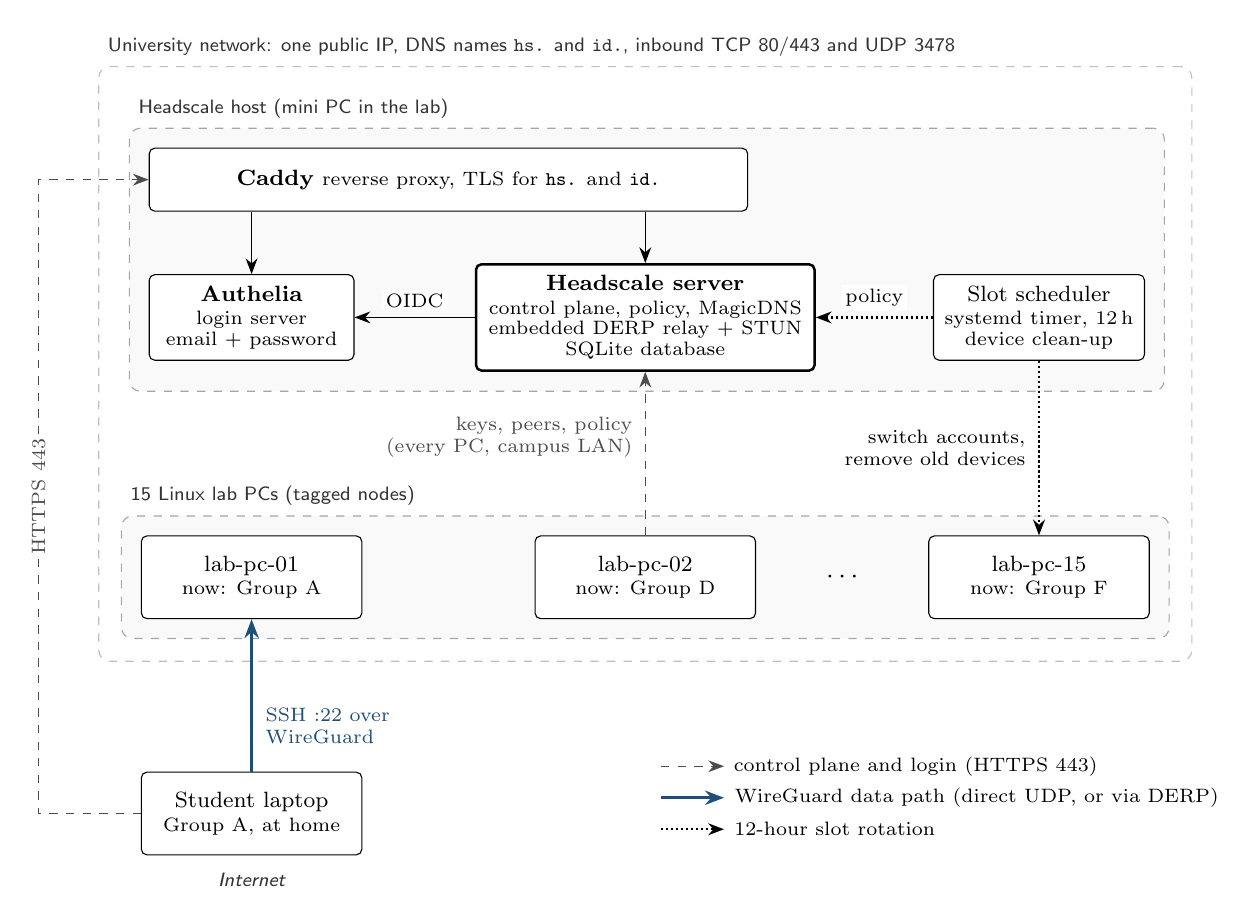
\begin{tikzpicture}
  % ---- Headscale host (mini PC) ----
  \node[box, minimum width=7.6cm, minimum height=0.8cm] (cd) at (2.5,1.75)
       {\textbf{Caddy}\ \scriptsize reverse proxy, TLS for \texttt{hs.} and \texttt{id.}};
  \node[box, minimum width=2.6cm] (pid) at (0,0)
       {\textbf{Authelia}\\[-1pt]\scriptsize login server\\[-2pt]\scriptsize email + password};
  \node[box, minimum width=4.3cm, line width=0.9pt] (hs) at (5,0)
       {\textbf{Headscale server}\\[-1pt]\scriptsize control plane, policy, MagicDNS\\[-2pt]\scriptsize embedded DERP relay + STUN\\[-2pt]\scriptsize SQLite database};
  \node[box, minimum width=2.6cm] (sc) at (10,0)
       {Slot scheduler\\[-1pt]\scriptsize systemd timer, 12\,h\\[-2pt]\scriptsize device clean-up};

  % ---- Lab PCs ----
  \node[box, minimum width=2.8cm] (p1)  at (0,-3.3)  {lab-pc-01\\[-1pt]\scriptsize now: Group A};
  \node[box, minimum width=2.8cm] (p2)  at (5,-3.3)  {lab-pc-02\\[-1pt]\scriptsize now: Group D};
  \node (dots) at (7.5,-3.3) {$\cdots$};
  \node[box, minimum width=2.8cm] (p15) at (10,-3.3) {lab-pc-15\\[-1pt]\scriptsize now: Group F};

  % ---- Student laptop (outside the campus) ----
  \node[box, minimum width=2.8cm] (lt) at (0,-6.3) {Student laptop\\[-1pt]\scriptsize Group A, at home};
  \node[zonelabel, font=\scriptsize\sffamily\itshape, below=3pt of lt] {Internet};

  % ---- Zones ----
  \begin{scope}[on background layer]
    \node[zone, fill=gray!5, fit=(cd)(pid)(hs)(sc)] (host) {};
    \node[zonelabel, anchor=south west] (hostlbl) at (host.north west) {Headscale host (mini PC in the lab)};
    \node[zone, fill=gray!5, fit=(p1)(p15)] (lab) {};
    \node[zonelabel, anchor=south west] (lablbl) at (lab.north west) {15 Linux lab PCs (tagged nodes)};
    \node[zone, draw=gray!50, inner sep=8pt, fit=(host)(lab)(hostlbl)(lablbl)] (uni) {};
    \node[zonelabel, anchor=south west] at (uni.north west)
         {University network: one public IP, DNS names \texttt{hs.} and \texttt{id.}, inbound TCP 80/443 and UDP 3478};
  \end{scope}

  % ---- Edges inside the host ----
  \draw[plain] (cd.south -| pid) -- (pid.north);
  \draw[plain] (cd.south -| hs)  -- (hs.north);
  \draw[plain] (hs.west) -- node[lbl, above=2pt]{OIDC} (pid.east);
  \draw[sched] (sc.west) -- node[lbl, above=2pt]{policy} (hs.east);

  % ---- Host to lab PCs (labels sit left of their lines, in empty space) ----
  \draw[ctrl]  (p2.north) -- node[lbl, left=3pt, align=right, pos=0.6]{keys, peers, policy\\(every PC, campus LAN)} (hs.south);
  \draw[sched] (sc.south) -- node[lbl, left=3pt, align=right]{switch accounts,\\remove old devices} (p15.north);

  % ---- Student laptop: login/control via Caddy, SSH straight to the PC ----
  \draw[ctrl]  (lt.west) -- ++(-1.3,0) coordinate (bend)
               -- node[lbl, rotate=90]{HTTPS 443} (bend |- cd.west) -- (cd.west);
  \draw[data]  (lt.north) -- node[lbl, right=3pt, align=left, pos=0.3]{SSH :22 over\\WireGuard} (p1.south);

  % ---- Legend ----
  \begin{scope}[shift={(5.2,-5.7)}, font=\scriptsize]
    \draw[ctrl]  (0,0)    -- (0.8,0)    node[right, black]{control plane and login (HTTPS 443)};
    \draw[data]  (0,-0.4) -- (0.8,-0.4) node[right, black]{WireGuard data path (direct UDP, or via DERP)};
    \draw[sched] (0,-0.8) -- (0.8,-0.8) node[right, black]{12-hour slot rotation};
  \end{scope}
\end{tikzpicture}
\caption{Pilot network architecture. Caddy is the only public entry point and
routes \texttt{hs.[uni-domain]} to Headscale and \texttt{id.[uni-domain]} to
Authelia. User traffic flows between laptop and lab PC, end-to-end encrypted
with WireGuard.}
\label{fig:arch}
\end{figure}

\textbf{How a connection is made.}
\begin{enumerate}[leftmargin=1.6em]
  \item Every device keeps an HTTPS (TCP 443) session to Headscale and
        receives only the peers the policy allows.
  \item A new connection starts out relayed through a DERP server. Meanwhile,
        both ends learn their public addresses via STUN (UDP 3478) and attempt
        NAT traversal.
  \item If a direct UDP path works, traffic moves to it (lowest latency).
        Under hard NAT, or where UDP is blocked, it stays on DERP over TCP 443,
        which is slower but works. The client keeps re-checking for a direct
        path.
  \item Every path is WireGuard-encrypted end to end. The relay only ever
        sees ciphertext.
\end{enumerate}

Our host runs Headscale's \textbf{embedded DERP relay}, so relayed traffic
stays on campus. Tailscale's public DERP servers stay in the map as a backup.
They can be removed to keep everything in-house, at the cost of a single point
of failure.

\textbf{One entry point.} Authelia's login page needs its own HTTPS hostname
next to Headscale's, but there is only one public IP and one port 443. Caddy
terminates TLS for both names with automatic Let's Encrypt certificates and
routes each name to its service. Headscale requires WebSocket support from a
reverse proxy, which Caddy provides; Headscale's maintainers say they do not
use proxies themselves, so the pilot tests this path early. STUN (UDP 3478)
goes straight to Headscale. Lab PCs reach the server on its campus LAN address
through a hosts-file entry, so they do not depend on the campus firewall
looping traffic back to the public IP (hairpin NAT).
For the same reason, the mini PC's own hosts file points \code{id.[uni-domain]}
at itself, so Headscale reaches Authelia locally when it checks a login.

\subsection{Machines, users and slots}

Each \textbf{lab PC} is registered once with a single-use pre-authorised key
that carries its tags (\code{tag:labpc} and its own \code{tag:pc-NN}). That
makes it a \emph{tagged node}, owned by the lab rather than by a person.
Hosted Tailscale could share a device into another tailnet by email, but
Headscale runs a single tailnet. Instead, every student is a user in our
tailnet, identified by their university email. A \textbf{thesis group} is a
list of emails in the access policy. ``Sharing'' a PC with a group is a policy
grant that exists only during the group's slot. As with Tailscale's shared
machines, the PC cannot start connections back to the students.

Each PC has 14 slots per week, \textbf{08:00--20:00} and
\textbf{20:00--08:00} every day. Each group gets two slots on different days
(Table~\ref{tab:slots}). At each boundary, a systemd timer on the host:
\begin{enumerate}[leftmargin=1.6em]
  \item writes the policy for the new slot from the schedule and roster files
        and reloads Headscale (\code{systemctl reload headscale}). All 15 PCs
        change in one batched update;
  \item removes the outgoing groups' devices from Headscale (Section~\ref{sec:nodes});
  \item logs in to each PC over SSH as the scheduler node, ends the outgoing
        group's sessions and processes, and moves the \code{slot-active} Linux
        group from the outgoing group's account to the incoming one;
  \item on any error, loads an admins-only policy and raises an alert, so
        access fails closed. Having no policy at all would allow everything.
\end{enumerate}

\begin{table}[H]
\centering\small
\caption{Example weekly schedule for one PC: six groups (A--F) and one
maintenance slot.}
\label{tab:slots}
\begin{tabular}{l*{7}{>{\centering\arraybackslash}p{1.1cm}}}
\toprule
 & Mon & Tue & Wed & Thu & Fri & Sat & Sun \\
\midrule
08:00--20:00 & A & C & E & A & C & E & \cellcolor{gray!15}\textit{maint.} \\
20:00--08:00 & B & D & F & B & D & F & \textit{spare} \\
\bottomrule
\end{tabular}
\end{table}

\noindent\begin{minipage}{\linewidth}
\begin{lstlisting}
"groups": { "group:thesis-a": ["s2101@[uni-domain]", "s2102@[uni-domain]", ...] },
"grants": [
  { "src": ["group:admins", "tag:scheduler"], "dst": ["tag:labpc"], "ip": ["tcp:22"] },
  // generated for the current slot (Mon 08:00-20:00): pc-01 shared with Group A
  { "src": ["group:thesis-a"], "dst": ["tag:pc-01"], "ip": ["tcp:22"] } ]
\end{lstlisting}
\end{minipage}

\textbf{Lab PCs.} Each PC runs Ubuntu LTS with the Tailscale client and plain
OpenSSH. Login is key-only, \code{AllowGroups lab-admins slot-active}
restricts who may log in, and the firewall accepts SSH only on
\code{tailscale0}. Each group has one Linux account holding its members' keys.
Home directories persist between slots, but running jobs stop at slot end, so
groups must checkpoint.

\subsection{Student login with Authelia}

We run our own login server, \textbf{Authelia}, on the mini PC. Headscale does
not check passwords itself: it hands student sign-in to Authelia over OIDC.
Authelia's documentation includes a Headscale setup, tested with Headscale
0.29.1.

\textbf{What the student does.} On the first day, the admin gives each student
their username and a starting password in private. At the start of each slot
the student:
\begin{enumerate}[leftmargin=1.6em]
  \item runs \code{tailscale login -{}-login-server}
        \code{https://hs.[uni-domain]}, or presses ``Log in'' in the Tailscale
        app. A browser tab opens on our login page at \code{id.[uni-domain]};
  \item enters their university email and password. The tab then reports
        success;
  \item connects with \code{ssh grp-a@lab-pc-01}, or with AnyDesk using the
        slot's password. This works only during their group's slot.
\end{enumerate}
Behind the scenes, Authelia tells Headscale ``this is s2101@[uni-domain], member
of \code{lab-pilot}''. Headscale registers the laptop under that email, and the
slot policy decides which PC, if any, it can reach. \emph{Signing in proves who
you are; the schedule decides what you can reach.} Students can keep a personal
Tailscale account alongside ours, because client 1.34 and later supports
several accounts.

\begin{itemize}[leftmargin=1.6em]
  \item \textbf{Accounts.} The admin adds each student to Authelia's user file
        with their university email and the group \code{lab-pilot}. Headscale
        admits only that group (\code{allowed\_groups}). Passwords are stored
        only as Argon2id hashes, never in plain text.
  \item \textbf{Password guessing.} Authelia's brute-force protection bans an
        account or IP address after repeated failed logins (by default, 3
        failures within 2 minutes trigger a 5-minute ban). We enable both
        modes.
  \item \textbf{Password resets.} The admin resets forgotten passwords, so no
        email server is needed. Self-service reset by email can be added later
        with an SMTP account. Two-factor codes (TOTP) can also be switched on
        later by changing the client's policy from \code{one\_factor} to
        \code{two\_factor}.
\end{itemize}

\noindent\begin{minipage}{\linewidth}
\begin{lstlisting}
users:                                    # Authelia user file: one entry per student
  s2101:
    displayname: "Student Name"
    email: "s2101@[uni-domain]"
    password: "$argon2id$v=19$m=65536,t=3,p=4$..."    # hash only, never the password
    groups: ["lab-pilot"]                 # Headscale: allowed_groups: ["lab-pilot"]
\end{lstlisting}
\end{minipage}

\textbf{Why not Google or University SSO.} Google sign-in depends on the
University's Google admin settings, which can block apps like ours, and a
personal Google project is limited to 100 test users. Our own login server
needs nothing from IT. Authelia's Headscale guide is community-maintained, so
the pilot first checks that Headscale receives each student's email and groups
correctly.

\subsection{Devices and node budget}
\label{sec:nodes}

A \emph{node} is a device, not a user: a student with a laptop and a phone is
two nodes. Each group has at least five students, and devices accumulate fast
if they stay registered (Table~\ref{tab:nodes}):

\begin{table}[H]
\centering\small
\caption{Nodes on the server (15 lab PCs and 1 scheduler included).}
\label{tab:nodes}
\begin{tabularx}{\textwidth}{Yp{2.6cm}p{2.4cm}}
\toprule
Situation & 1 device / student & 2 devices / student \\
\midrule
One slot, all 15 PCs in use, 5 students per group & 91 & 166 \\
Devices kept all week (6 groups per PC, 90 groups) & 466 & 916 \\
\bottomrule
\end{tabularx}
\end{table}

Headscale's FAQ says it ``can likely handle 100s of devices (maybe more)''
when the network changes rarely, because every change rebuilds the network map
for every node. We therefore keep \textbf{only the current slot's devices} on
the server:
\begin{itemize}[leftmargin=1.6em]
  \item At slot end the scheduler deletes the outgoing groups' devices.
        Students sign in again with their password at the start of their next
        slot, which takes a few seconds.
  \item Every five minutes, a clean-up job removes devices of students who are
        not in an active slot, and any device beyond \textbf{two per student}.
\end{itemize}
The server then holds at most about \textbf{166 nodes} (91 with one device per
student) instead of 466--916. Student \emph{accounts} grow with the roster,
but accounts are only database rows and do not affect performance. The main
load is the slot changeover twice a day, when up to about 150 devices leave
and rejoin. The pilot measures how long that takes.

\subsection{Remote desktop in the slot (AnyDesk)}

AnyDesk is how groups work today, and it is where the slots are bypassed. It
stays available, but only inside the slot. There are two caveats.
\begin{enumerate}[leftmargin=1.6em]
  \item AnyDesk normally connects through \emph{AnyDesk's own servers}, not
        our tailnet, so the Headscale policy cannot block it. Instead, the
        AnyDesk password becomes the slot key. At every slot change the
        scheduler sets a new unattended-access password
        (\code{anydesk -{}-set-password}, from AnyDesk's Linux CLI), gives it
        only to the incoming group, and restarts AnyDesk to drop the outgoing
        session. The old password stops working the moment the slot ends. The
        PC's desktop login also switches to the incoming group's account.
  \item AnyDesk's free licence is for private use only. Lab use counts as
        professional and needs a paid licence.
\end{enumerate}
If no licence is available, \textbf{RustDesk} (open source) can connect
directly to the PC's tailnet address. The same slot policy then controls it,
just like SSH.

% ---------------------------------------------------------------------------
\section{Technical Specifications}

The whole system runs on one small, low-power machine in the lab (Table~\ref{tab:host}).

\begin{table}[H]
\centering\small
\caption{Headscale host: hardware and power.}
\label{tab:host}
\begin{tabularx}{\textwidth}{P{3.1cm}Y}
\toprule
Machine & Intel N100-class mini PC (4 cores), 8\,GB RAM, 128--256\,GB SSD, 1\,GbE wired \\
Software & Ubuntu Server 24.04 LTS; Headscale (latest stable release, pinned) with SQLite and embedded DERP; Authelia; Caddy; slot scheduler (systemd timer and script) \\
Power draw & N100 mini PCs measure about 6--12\,W idle and 22--29\,W at full load; about 7\,kWh per month at a 10\,W average. We will measure our unit \\
Backup power and data & 650\,VA UPS. A nightly copy of the Headscale and Authelia databases, user file, keys and configuration goes to a second disk \\
\bottomrule
\end{tabularx}
\end{table}

Section~\ref{sec:uni} lists the ports exposed to the internet. On the lab PCs,
SSH (TCP 22) is accepted only on the \code{tailscale0} interface.

% ---------------------------------------------------------------------------
\section{What We Need from the University}
\label{sec:uni}

\begin{enumerate}[leftmargin=1.6em]
  \item \textbf{One static public IPv4 address}, routed or forwarded to the
        mini PC.
  \item \textbf{Two DNS records} for that address: \code{hs.[uni-domain]}
        (Headscale) and \code{id.[uni-domain]} (login server).
  \item \textbf{Three inbound ports open from the internet} to that address,
        and no others:
\end{enumerate}

\begin{table}[H]
\centering\small
\caption{Ports exposed to the internet (inbound to the public IP only).}
\label{tab:exposed}
\begin{tabularx}{\textwidth}{P{1.8cm}P{2.3cm}YP{2.5cm}}
\toprule
Port & Received by & Purpose & Status \\
\midrule
TCP 443 & Caddy & Student login (Authelia), Tailscale control traffic to Headscale, and the DERP relay & Required \\
UDP 3478 & Headscale & STUN, so devices can find their public address and connect directly & Required \\
TCP 80 & Caddy & Let's Encrypt certificate checks; redirects browsers to HTTPS & Recommended\textsuperscript{*} \\
\bottomrule
\end{tabularx}

\raggedright\footnotesize\textsuperscript{*}Caddy can also validate certificates over TCP 443, so port 80 can stay closed if the University prefers.
\end{table}

\textbf{Nothing else is exposed.} The lab PCs, SSH (port 22) and the Headscale
and Authelia services themselves are not reachable from the internet. All
student traffic reaches a PC only through Caddy (login and control) or
WireGuard (SSH), and only during the group's slot.

\textbf{Outbound traffic from the lab network}, which campus networks normally
already allow: UDP 41641, UDP 3478 and TCP 443 to any address, from the lab PCs
and the mini PC. If outbound UDP is blocked, connections still work through our
relay on TCP 443, only slower. AnyDesk keeps using the outbound connections it
uses today.

The project team provides everything else: hardware, software, certificates,
student accounts, PC setup and operation.

% ---------------------------------------------------------------------------
\section{Risks}

\begin{table}[H]
\centering\footnotesize
\begin{tabularx}{\textwidth}{P{5.0cm}Y}
\toprule
Risk & Mitigation \\
\midrule
Scheduler fails at a slot boundary & Falls back to an admins-only policy (no student access) and alerts the admins \\
Slot changeover is slow (about 150 devices leave and rejoin) & Devices are removed in one batch; changeover time is measured in the pilot; device limit can drop to one per student \\
Authelia is down & Already-connected devices keep working; only new sign-ins wait. Authelia is backed up nightly \\
A password is guessed or shared & Brute-force bans; the admin resets the password; two-factor codes can be switched on; a stolen login still reaches only that group's PC during its slot \\
AnyDesk bypasses the tailnet & The password is rotated and the session ended at every boundary; licensed use only, or RustDesk over the tailnet \\
Headscale host fails & UPS and nightly backups; existing tunnels survive short outages \\
\bottomrule
\end{tabularx}
\end{table}

\end{document}
